\documentclass[11pt]{beamer}
\usepackage[utf8]{inputenc}
\usepackage[T1]{fontenc}
\usepackage{amsmath,amssymb}
\usepackage{amsfonts}
\usepackage{paralist}
\usepackage{color}
\usepackage{graphicx}
\usepackage{pgfplots}
%\usepackage{authblk}
\usepackage{url}
\usepackage{multirow}
\usepackage{booktabs}
\usepackage{blindtext}
\usepackage{adjustbox}
\usepackage{subcaption}

\mode<presentation> {
	\usetheme{Berlin}
	\usecolortheme{default}}

\title{Final Basic Cloud Assigment}
\author{Valentinis Alessio}
\institute{Università degli Studi di Trieste}
\date{21st march 2024}

\begin{document}
\begin{frame}
	\titlepage
\end{frame}

\begin{frame}{About the assignment}
	The goal of the Exercise was to deploy a Cloud based file storage system, using containerization, in particular Docker and Docker-compose, with the following requirements:
	\begin{itemize}
		\item Seamless implementation of file storage for users;
		\item Role Authentication policy
		\item Testing of the platform
		\item Discuss security measures
		\item Assess scalability
	\end{itemize}
\end{frame}

\begin{frame}{Nextcloud approach}
	I approached the problem using Nextcloud, an application software that allows for an out-of-the-box implementation of almost all the requirements of the project, such as:
	\begin{itemize}
		\item Flexible storage solution, allowing for both Object Based and NFS Storage System.
		\item Custom backend database solutions
		\item Esaye implementation of caching system
		\item Role based access
		\item Wide range of customizable security features
		\item Docker image for simple dockerized deployement
	\end{itemize}
\end{frame}

\begin{frame}{Security features}
	Nextcloud offers by default a great number of customizable features regarding security, such as:
	\begin{itemize}
		\item Server Side Encryption
		\item Personalizable Password settings
		\item Two-Factor authentication
		\item Seamless proxy integration
	\end{itemize}
\end{frame}

\begin{frame}{Deployement}
	\begin{itemize}
		\item The deployement of this enivronment is done using Docker-compose
		\item All features are manageable from the UI, including a basic but quite complete monitoration of the system
		\item Vast ecosystem of applications that enable for huge personalization of the service.
	\end{itemize}
	\begin{figure}
		\centering
		\begin{subfigure}{0.35\textwidth}
			\centering
			\label{fig:docker-compose}
			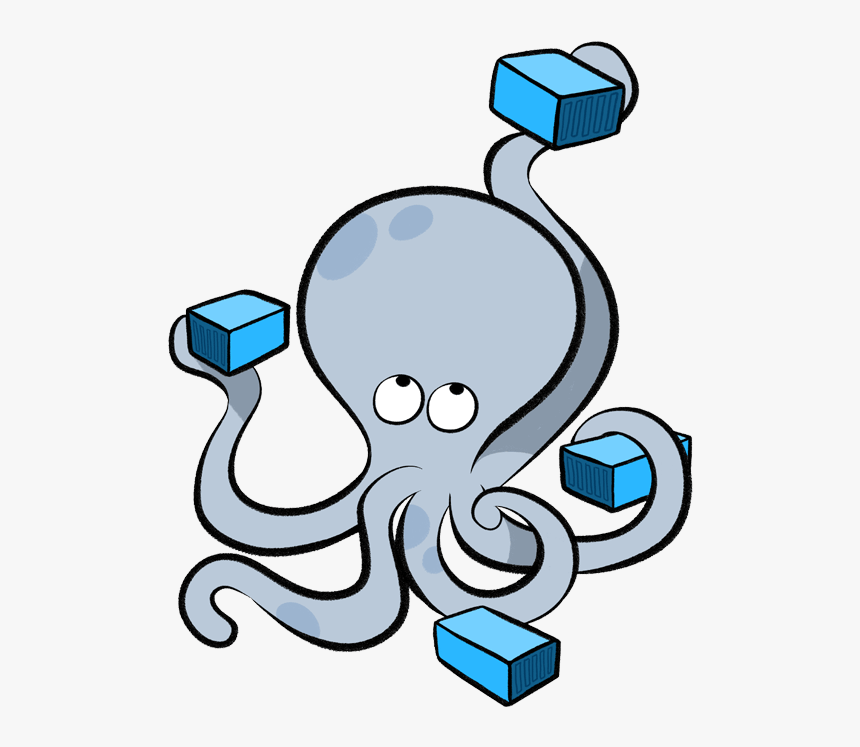
\includegraphics[width=0.7\linewidth]{docker-compose}
		\end{subfigure}
		\begin{subfigure}{0.35\textwidth}
			\centering
			
\includegraphics[width=0.7\linewidth]{nextcloud}
			\label{fig:nextcloud}
		\end{subfigure}
	\end{figure}
\end{frame}

\begin{frame}{Testing}
	To test the deployement I used the library Locust, written in Python.
	\begin{figure}[h]
		\begin{subfigure}{0.4\textwidth}
		\centering
		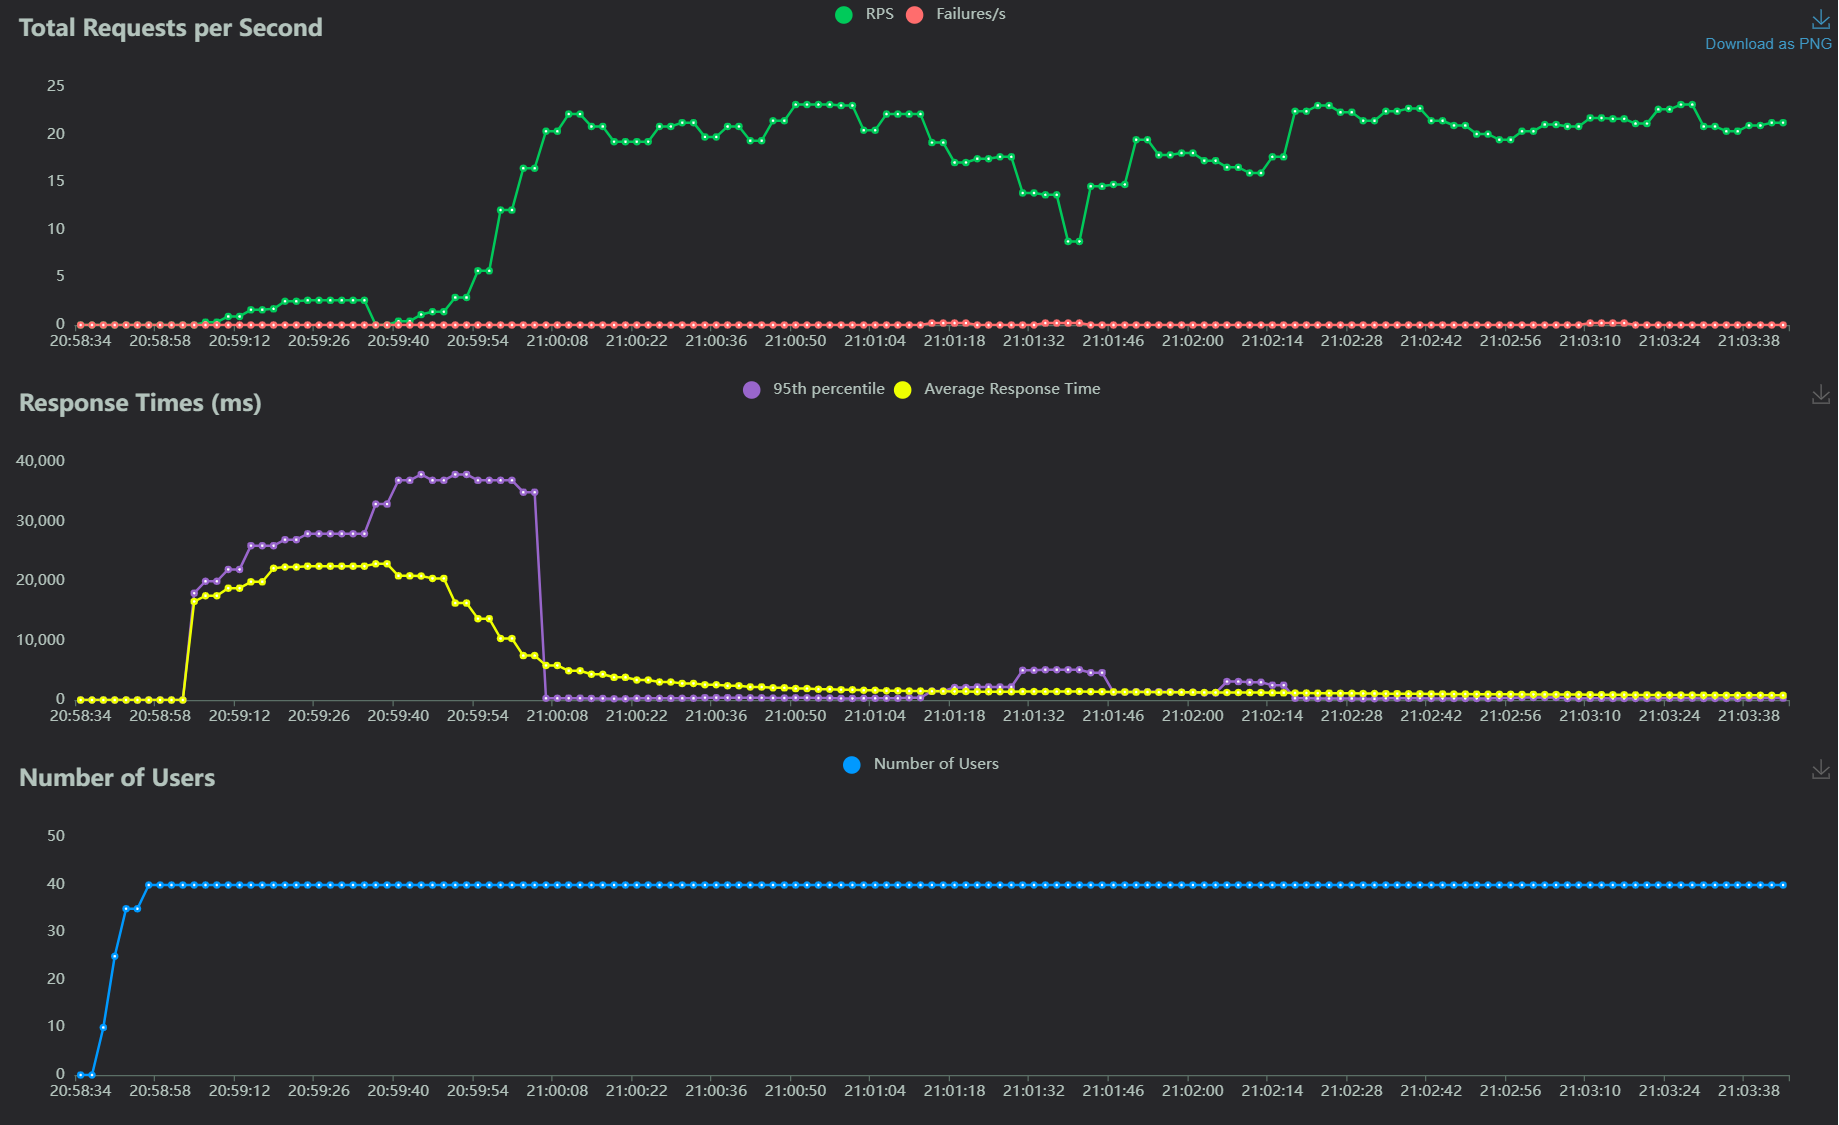
\includegraphics[width=0.95\linewidth]{../report/total_requests_per_second_40user1mb}
		\caption{Load test for medium-sized files, 40 users.}
		\end{subfigure}
		\begin{subfigure}{0.45\textwidth}
		\label{fig:totalrequestspersecond40user1mb}
		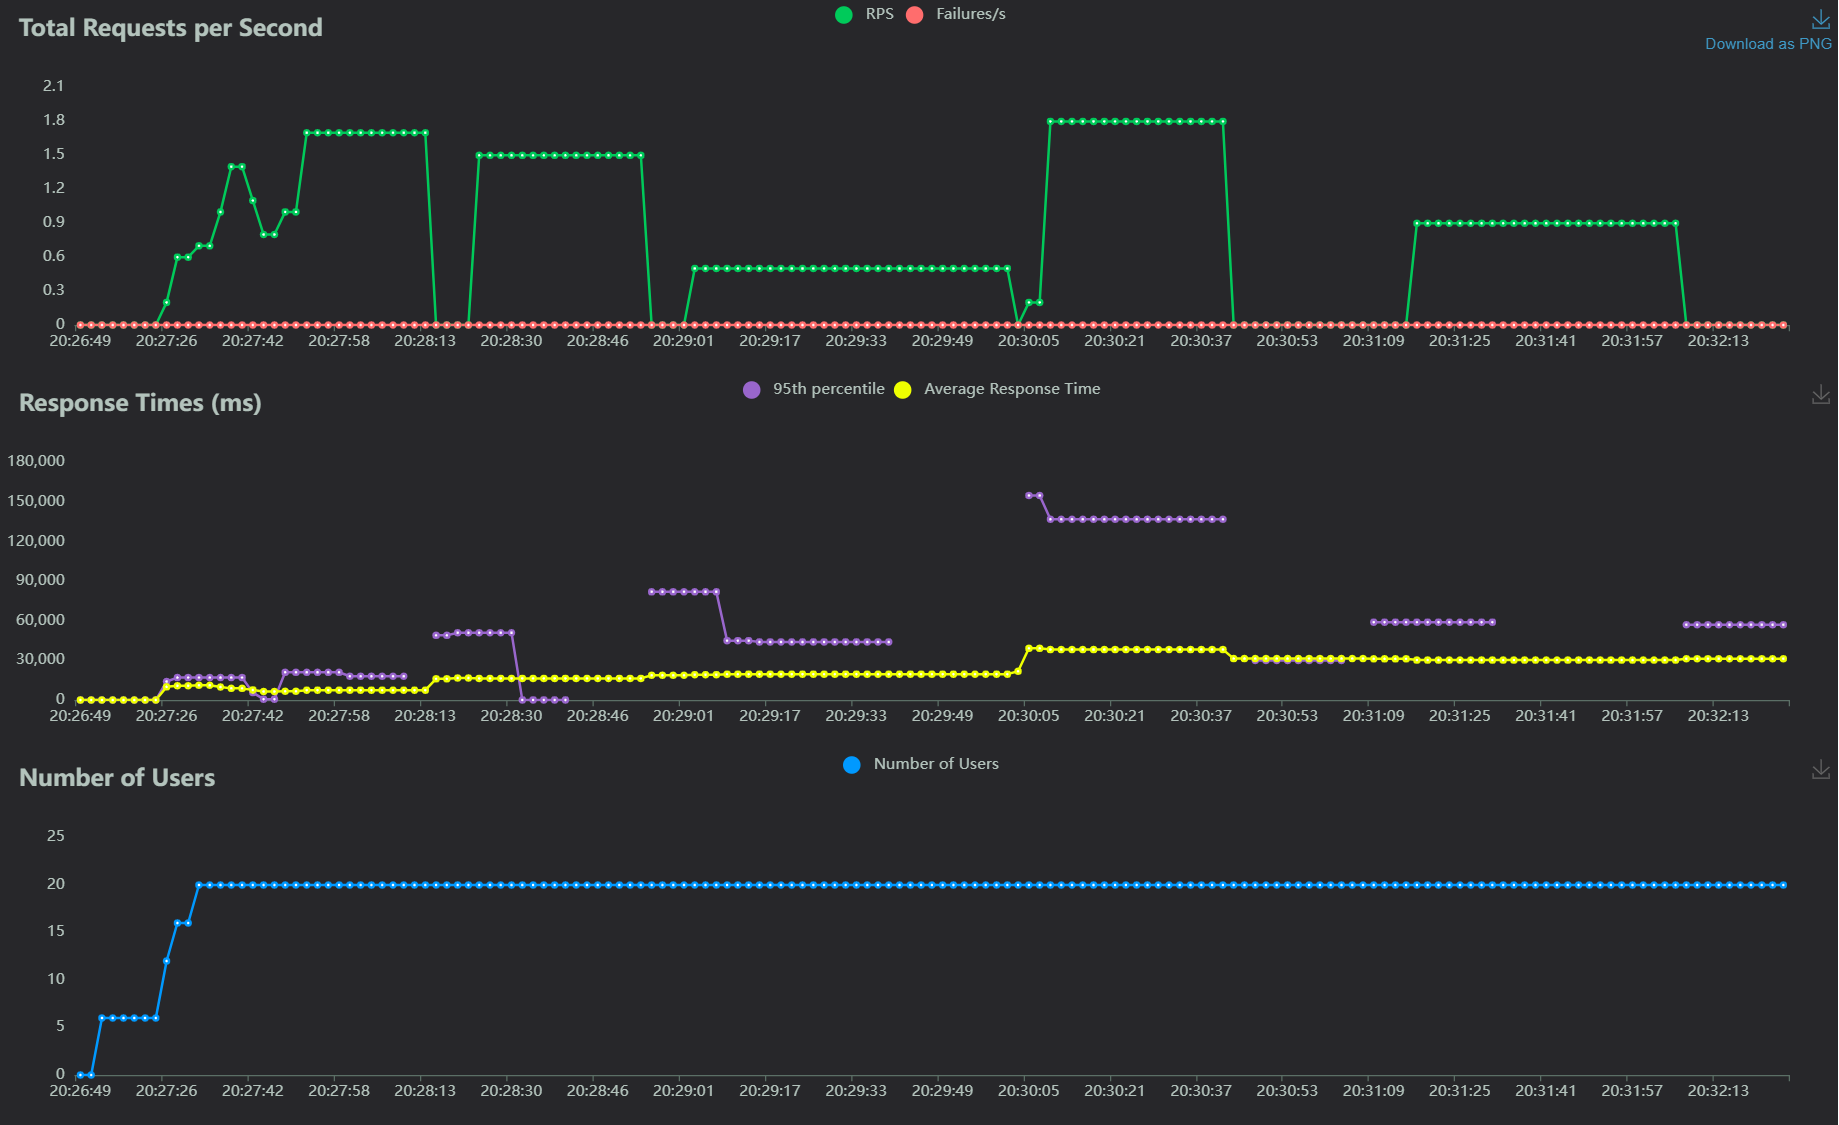
\includegraphics[width=0.9\linewidth]{../report/response_times_(ms)_20users_1gb}
		\caption{Load test for large size files, 20 users.}
		\label{fig:responsetimesms20users1gb}
		\end{subfigure}
	\end{figure}
\end{frame}

\begin{frame}{Scalability analysis}
	In this section, I analyzed two possible scalable deployements solutions, namely:
	\begin{itemize}
		\item On-premise deployement on a NFS or Storage Server.
		\item Cloud deployement, with authomatic scaling.
	\end{itemize}
\end{frame}

\begin{frame}{Deployement on exixting infrastructure}
	Deployement of Nextcloud on an existing centralized or distributed File System.
	
	\textbf{Main aspects}
	\begin{itemize}
		\item Infrastructure control
		\item Personalization
		\item Cost
		\item Security
		\item Data location
	\end{itemize}
\end{frame}

\begin{frame}{Cloud deployement}
	Deployement of Nextcloud using a Cloud Object Storage System (Amazon S3).
	\begin{itemize}
		\item Cloud database solution
		\item Scalability
		\item Service management
		\item World Wide Availability
		\item Cost efficiency
	\end{itemize}
\end{frame}

\begin{frame}{Cost efficiency evaluations}
	\textbf{Deployement on existing infrastructure}
	\begin{itemize}
		\item Higher initial costs, but lower maintenance and operational costs
		\item Affordable if you know in advance what you traffic will be, managin the infrastructure accordingly
	\end{itemize}
	
	\textbf{Cloud Deployement}
	\begin{itemize}
		\item Almost zero initial costs, with operational costs depending on the demand
		\item Convenient for little installations and for situations with fluctuating traffic
	\end{itemize}
\end{frame}

\end{document}